\subsection{Прямоугольная функция}

Рассмотрим семейство функций 
\begin{equation}
    f(t) = \begin{cases}
        a, & |t| \le b, \\
        0, & |t| > b
    \end{cases}
    \label{eq:rectangle_function}
\end{equation}

\subsubsection{Графики исходных функций}
Графики данной функции при различных значениях $a$ и $b$ представлены на рисунках \ref{fig:rectangle_1}, \ref{fig:rectangle_2} и \ref{fig:rectangle_3}.

\begin{figure}[ht!]
    \centering
    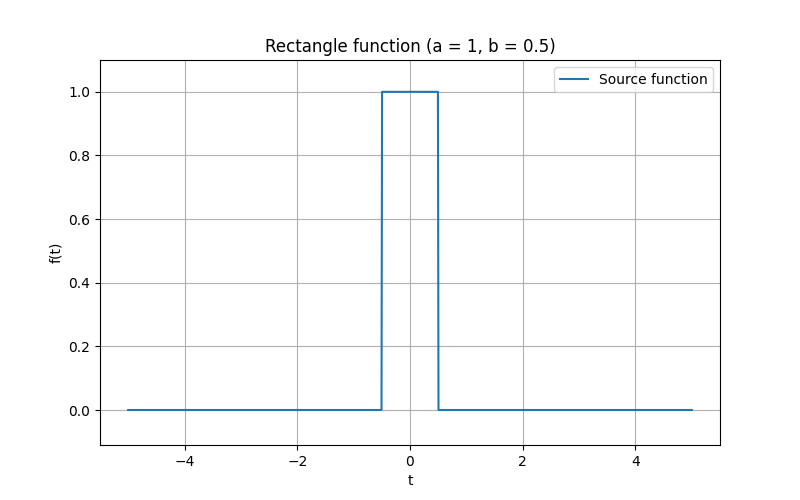
\includegraphics[width=\textwidth]{media/rectangle_1.png}
    \caption{График прямоугольной функции $f(t)$ при $a = 1$, $b = 0.5$}
    \label{fig:rectangle_1}
\end{figure}

\begin{figure}[ht!]
    \centering
    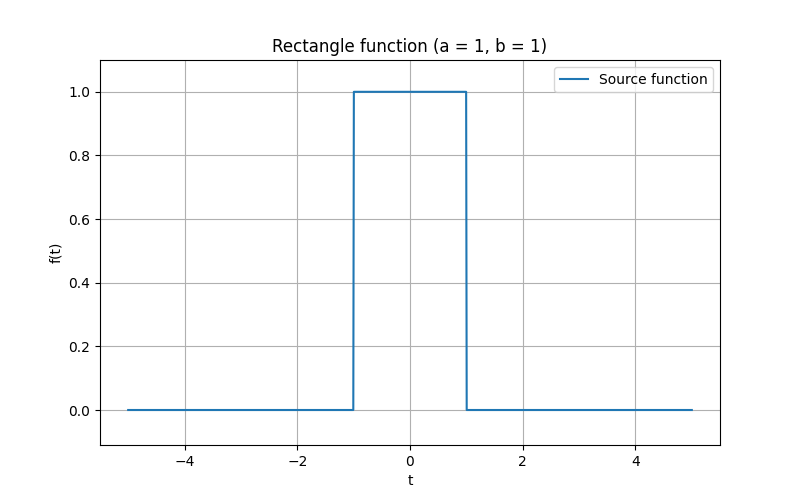
\includegraphics[width=\textwidth]{media/rectangle_2.png}
    \caption{График прямоугольной функции $f(t)$ при $a = 1$, $b = 1$}
    \label{fig:rectangle_2}
\end{figure}

\begin{figure}[ht!]
    \centering
    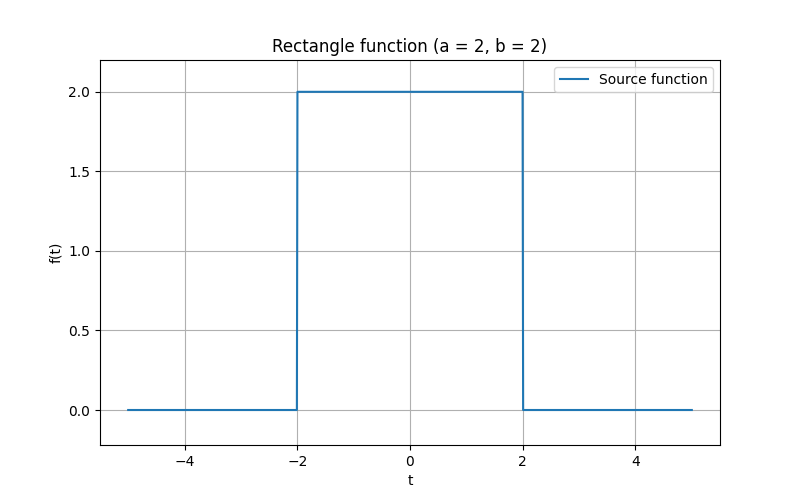
\includegraphics[width=\textwidth]{media/rectangle_3.png}
    \caption{График прямоугольной функции $f(t)$ при $a = 2$, $b = 2$}
    \label{fig:rectangle_3}
\end{figure}

\subsubsection{Нахождение образа функции}
Согласно формуле \eqref{eq:image_from_function}, Фурье образ функции $f(t)$ задается следующим выражением:
\begin{equation}
    \hat{f}(\omega) = \frac{1}{\sqrt{2\pi}} \int_{-\infty}^{\infty} f(t) e^{-i\omega t} dt = \frac{1}{\sqrt{2\pi}} \int_{-b}^{b} a e^{-i\omega t} dt = \frac{a}{-\omega i\sqrt{2\pi}} e^{-i\omega t} \Biggr|_{-b}^{b} = \frac{a(e^{i\omega b} - e^{-i\omega b})}{\omega i \sqrt{2 \pi}}
\end{equation}

Применив формулу Эйлера, получим:
\begin{equation}
    \hat{f}(\omega) = \frac{2ab}{\sqrt{2\pi}}\sinc(\omega b)
    \label{eq:rectangle_image}
\end{equation}

для $a = 1$, $b = 0.5$:
\begin{equation}
    \hat{f_1}(\omega) = \frac{1}{\sqrt{2\pi}}\sinc(\omega / 2)
\end{equation}

для $a = 1$, $b = 1$:
\begin{equation}
    \hat{f_2}(\omega) = \frac{2}{\sqrt{2\pi}}\sinc(\omega)
\end{equation}

для $a = 2$, $b = 2$:
\begin{equation}
    \hat{f_3}(\omega) = \frac{8}{\sqrt{2\pi}}\sinc(2\omega)
\end{equation}

\subsubsection{Графики образов функций}
Графики образов прямоугольной функции при различных значениях $a$ и $b$ представлены на рисунках \ref{fig:rectangle_1_image}, \ref{fig:rectangle_2_image} и \ref{fig:rectangle_3_image}.

\begin{figure}[ht!]
    \centering
    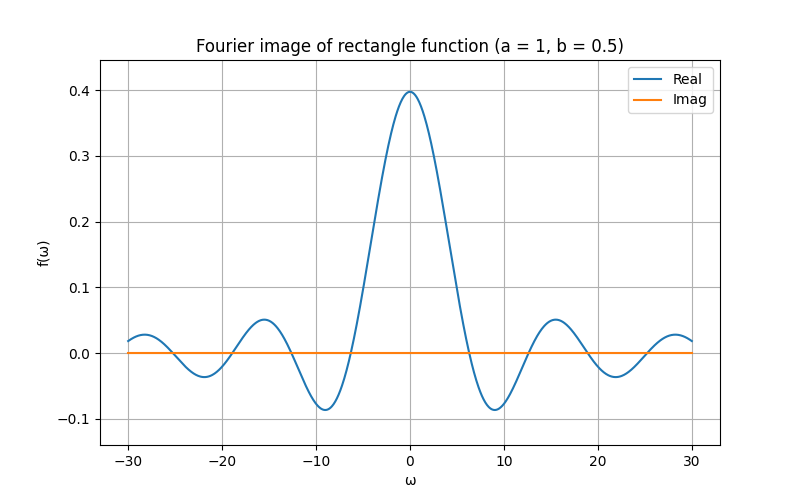
\includegraphics[width=\textwidth]{media/rectangle_1_image.png}
    \caption{График преобразования Фурье $\hat{f_1}(\omega)$ прямоугольной функции $f(t)$ при $a = 1$, $b = 0.5$}
    \label{fig:rectangle_1_image}
\end{figure}

\begin{figure}[ht!]
    \centering
    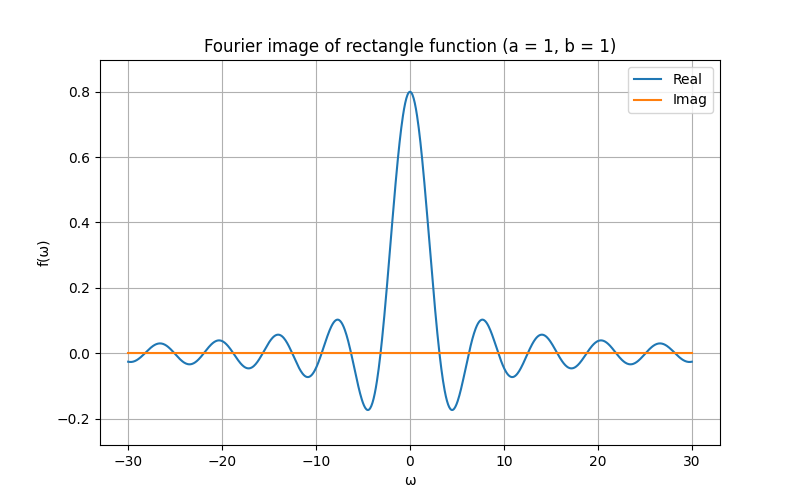
\includegraphics[width=\textwidth]{media/rectangle_2_image.png}
    \caption{График преобразования Фурье $\hat{f_2}(\omega)$ прямоугольной функции $f(t)$ при $a = 1$, $b = 1$}
    \label{fig:rectangle_2_image}
\end{figure}

\begin{figure}[ht!]
    \centering
    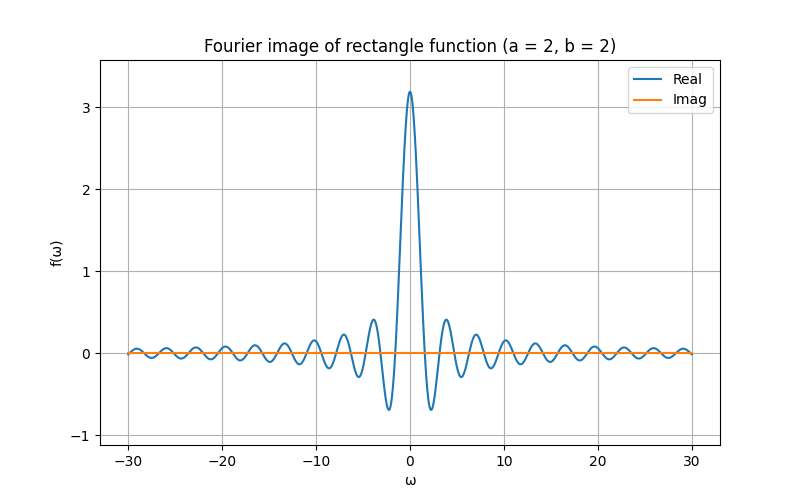
\includegraphics[width=\textwidth]{media/rectangle_3_image.png}
    \caption{График преобразования Фурье $\hat{f_3}(\omega)$ прямоугольной функции $f(t)$ при $a = 2$, $b = 2$}
    \label{fig:rectangle_3_image}
\end{figure}

\FloatBarrier
\subsubsection{Проверка равенства Парсеваля}
Проверим равенство Парсеваля (см. формулу~\eqref{eq:parseval_indentity}). Для этого воспользуемся функцией \texttt{parseval\_check}. 
% table with parseval check results
\begin{table}[ht!]
    \centering
    \begin{tabular}{|c|c|}
        \hline
        $\displaystyle\int_{-100}^{100}{|f(t)|^2}$ & $\displaystyle\int_{-100}^{100}{|\hat{f_1}(\omega)|^2}$ \\
        \hline
        1.00010 & 0.99376 \\
        \hline
    \end{tabular}
    \caption{Результаты проверки равенства Парсеваля для прямоугольной функции $f(t)$ при $a = 1$, $b = 0.5$}
    \label{tab:rectangle_1_parseval_check}
\end{table}

\begin{table}[ht!]
    \centering
    \begin{tabular}{|c|c|}
        \hline
        $\displaystyle\int_{-100}^{100}{|f(t)|^2}$ & $\displaystyle\int_{-100}^{100}{|\hat{f_2}(\omega)|^2}$ \\
        \hline
        2.00020 & 1.99386 \\
        \hline
    \end{tabular}
    \caption{Результаты проверки равенства Парсеваля для прямоугольной функции $f(t)$ при $a = 1$, $b = 1$}
    \label{tab:rectangle_2_parseval_check}
\end{table}

\begin{table}[ht!]
    \centering
    \begin{tabular}{|c|c|}
        \hline
        $\displaystyle\int_{-100}^{100}{|f(t)|^2}$ & $\displaystyle\int_{-100}^{100}{|\hat{f_3}(\omega)|^2}$ \\
        \hline
        16.00160 & 15.97619 \\
        \hline
    \end{tabular}
    \caption{Результаты проверки равенства Парсеваля для прямоугольной функции $f(t)$ при $a = 2$, $b = 2$}
    \label{tab:rectangle_3_parseval_check}
\end{table}

Видим, что во всех случаях значения почти не отличаются друг от друга. Различие, по большей части, обусловлено тем, что в программе нельзя найти интеграл по бесконечности, поэтому просто берется достаточно большой интервал интегрирования.

\subsubsection{Анализ результатов}
Влияние параметров $a$ и $b$ на графики прямоугольной функции и ее образа можно понять из соответствующих формул (см. формулы~\eqref{eq:rectangle_function} и~\eqref{eq:rectangle_image}).
В исходной функции $f(t)$ параметр $a$ отвечает за высоту прямоугольника, а $b$ за его ширину.
В образе $\hat{f}(\omega)$ параметр $a$ отвечает за амплитуду колебаний, а $b$ за частоту колебаний.

Принцип неопределенности Гейзенберга утверждает, что нельзя одновременно точно определить положение и импульс частицы. В данном случае, чем меньше ширина прямоугольника, тем больше ширина его образа, и наоборот. 
